\documentclass[12pt,a4paper]{article}
\usepackage[utf8]{inputenc}
\usepackage[german]{babel}
\usepackage[T1]{fontenc}
\usepackage{amsmath}
\usepackage{amsfonts}
\usepackage{amssymb}
\usepackage{graphicx}
\usepackage{float}
\usepackage[left=2cm,right=2cm,top=2cm,bottom=2cm]{geometry}
\usepackage{siunitx}
\author{Moritz}

\begin{document}
\setlength{\parindent}{0pt} 
\begin{center}
{\LARGE Versuchsprotokoll}\\
\begin{large}
zum Grundpraktikum Physik Teil I\\[0.4cm]
an der RWTH Aachen\\
I. Physikalisches Institut B\\[4.5cm]
\Large\textbf{\textsl{Mechanik}}\\[4cm]
\normalsize\textit{vorgelegt\\von}\\[0.4cm]
\large{Moritz Berger\\Tim Herbermann\\Gerald Kolter\\Sebastian Siebert}\\[1cm]
\large \textit{Gruppe B07} \\ [3cm]
\large \textbf{Wintersemester 2016/2017}
\end{large}
\end{center}
\newpage

\tableofcontents
\newpage

\part{Trägheitsmomente}

\section{Grundlagen}
In diesem Versuch soll das Trägheitsmoment verschiedener Körper analysiert werden.\\
Dieses ist allgemein definiert über
\begin{equation}
J = \int r^2 dm.
\end{equation}
Wir werden das Trägheitsmoment aus der Schwingungsdauer einer Drillachse, die durch eine Spiralfeder zum schwingen gebracht wird, bestimmen. Dabei wird ein Zusammenhang zwischen Schwingungsperiode T und dem Trägheitsmoment J  aus der Definition des Drehmomentes M hergeleitet:
\begin{equation}
M = J\cdot \dot{\omega}\Rightarrow -D\cdot \phi = J\cdot \ddot{\phi}\Rightarrow \ddot{\phi} + \dfrac{D}{J}\cdot \phi = 0
\end{equation}
Die Lösung dieser Differentialgleichung ist eine harmonische Schwingung mit der Kreisfrequenz $\omega = \sqrt{\dfrac{D}{J}}$. Daraus folgt:
\begin{equation}
 T = 2\cdot \pi \sqrt{\dfrac{J}{D}}
\end{equation}
oder, falls man das Trägheitsmoment angeben möchte:
\begin{equation}
J = \dfrac{D}{4\cdot \pi^2}\cdot T^2
\label{eq:Trägheitsmoment}
\end{equation}\\
\\
Der Versuch wird in drei Teile aufgeteilt.\\
Im ersten Teil soll das Trägheitsmoment von Massenpunkten in Abhängigkeit von dem Abstand zur Drehachse untersucht werden. Dabei wird als erstes das Direktionsmoment der Feder bestimmt.\\
Im zweiten Teil wird das Trägheitsmoment eines Hohlzylinders, eines Vollzylinders, einer Kugel und einer Kreisscheibe miteinander verglichen.\\
Im dritten Teil soll der Steinersche Satz
\begin{equation}
J = J_0+m \cdot R^2
\end{equation}
bestätigt werden.

\section{Aufbau und Durchführung}
\begin{figure}
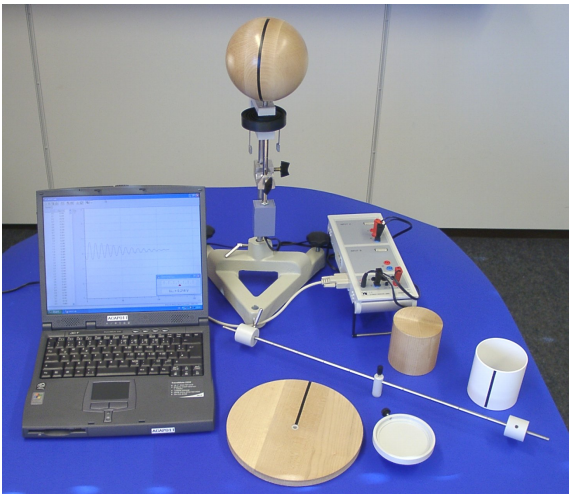
\includegraphics[width=\linewidth]{Bilder/Aufbau.PNG}
\caption{Versuchsaufbau für die Bestimmung von Trägheitsmomenten}
\label{fig:Aufbau}
\end{figure}
Der grundsätzliche Aufbau aller drei oben erwähnten Teilversuche ist gleich. Er wird in Abbildung \ref{fig:Aufbau} dargestellt. Es wird ein kugelgelagterter Stab mit einem Stativ und mit einer Spiralfeder, die eine Schwingung erzeugen soll, befestigt. Auf den Stab können je nach Teilversuch verschiedene Aufsätze aufgesetzt werden, deren Trägheitsmoment gemessen wird. Am unteren Stabende werden an der Innenseite einer U-förmigen Gabel zwei Magnete so befestigt, dass sich Nord- und Südpol gegenüber liegen. Zwischen die Magnete wird eine Hallsonde geführt, die als Winkelaufnehmer dient. Sie wird mit der Spannungsquelle des CASSYs verbunden. Die entstehende Hall-Spannung wird ebenfalls mit dem CASSY gemessen. Vor dem Experimentieren wird die Hallsonde durch horizontales Drehen so justiert, dass die gemessene Spannung möglichst bei \SI{0}{V} liegt. \\
Alle Experimente wurden mit zwei Aufbauten durchgeführt. Dabei hatte ein Aufbau die Feder mit der Nummer 2 und der andere Aufbau Feder Nummer 3. Entsprechend wird im Folgenden auf die Aufbauten bzw. Federn verwiesen.


\section{Bestimmung des Direktionsmomentes}

\begin{figure}
\begin{center}
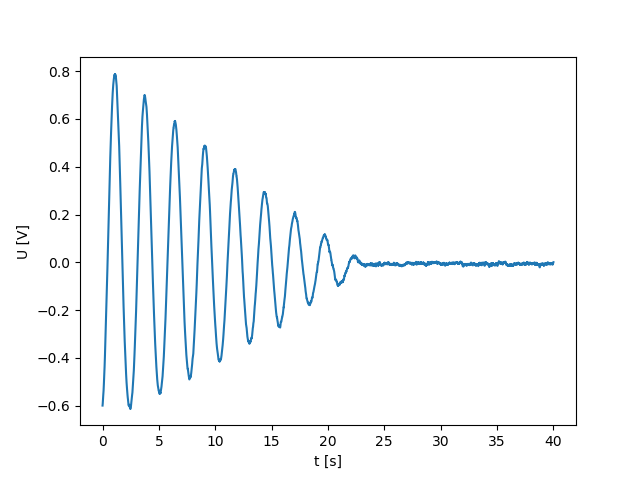
\includegraphics[scale=0.5]{Bilder/Feder2Kerbe1}
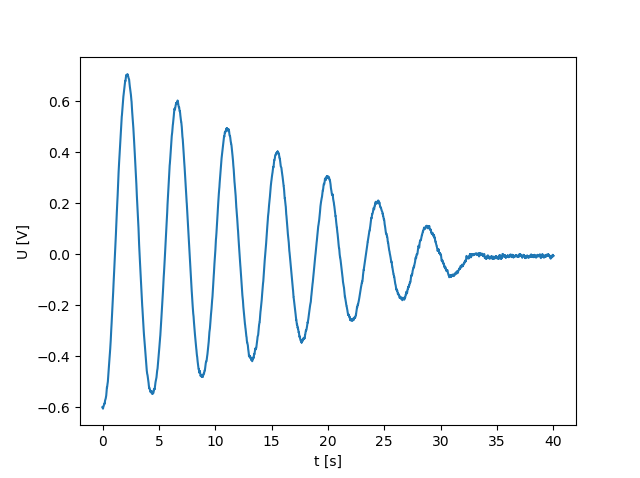
\includegraphics[scale=0.5]{Bilder/Feder2Kerbe3}
\end{center}
\caption{Exemplarische Schwingungsverläufe für Gewichte auf der ersten und dritten Kerbe für Feder 2.}
\label{fig:RohdatenFeder2}
\end{figure}

\begin{figure}
\begin{center}
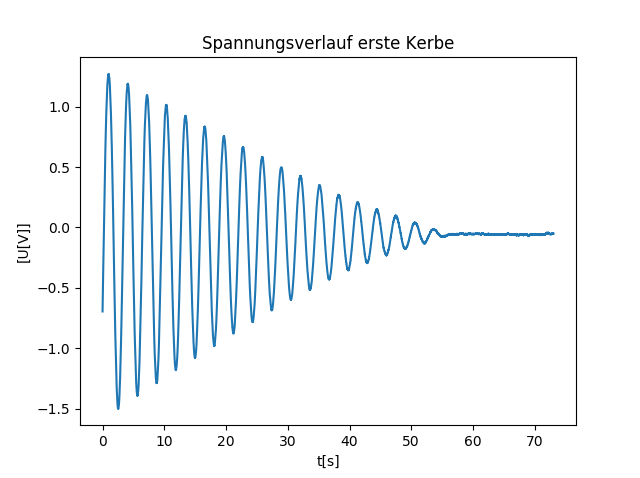
\includegraphics[scale=0.5]{Bilder/Feder3Kerbe1}
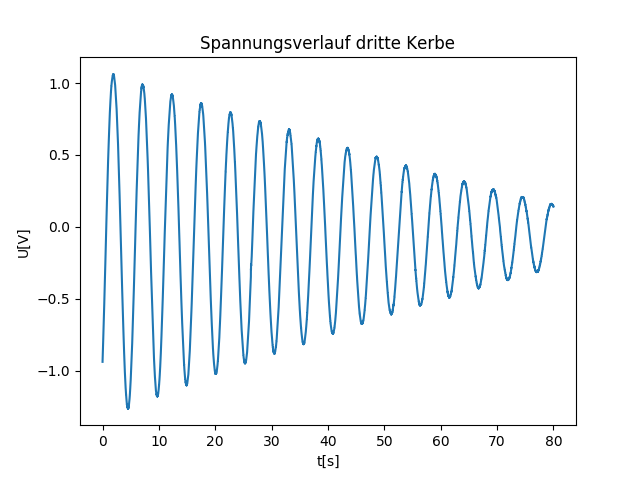
\includegraphics[scale=0.5]{Bilder/Feder3Kerbe3}
\end{center}
\caption{Exemplarische Schwingungsverläufe für Massenpunkte auf der ersten und dritten Kerbe für Feder 3.}
\label{fig:RohdatenFeder3}
\end{figure}


Einige exemplarische Schwingungsverläufe finden sich in Abbildung [hier Rohdaten Feder 2] für Feder 2 und in Abbildung \ref{fig:RohdatenFeder3} für Feder 3.\\

Vor Aufzeichnung der Schwingungsvorgänge wurden die beiden Kugeln gewogen sowie der Kerbenabstand bestimmt. Die ausgewiesenen statistischen Fehler ergeben sich aus der Ablesegenauigkeit, der systematische Fehler der Waage wurde auf \SI{0.1}{g} abgeschätzt. Der systematische Fehler des Maßbands ist durch die Güteklasse II gegeben. Die Ergebnisse beider Federn finden sich in Tabelle \ref{tab:Vormessungen}.\\


\begin{table}
\caption{Vormessungen zur Bestimmung des Direktionsmoments der Federn.}
\begin{center}
\begin{tabular}{|c|c|c|c|c|}
\hline
Feder & $m_1$[g] & $m_2$[g] & Kerbenabstand $d$[cm]\\
\hline
2 & 237.8 $\pm$ 0.03 $\pm$ 0.1 & 238.2 $\pm$ 0.03 $\pm$ 0.1 & 5.00 $\pm$ 0.03 $\pm$ 0.07 \\
\hline
3 & 238.50 $\pm$ 0.03 $\pm$ 0.1 & 238.40 $\pm$ 0.03 $\pm$ 0.1 & 4.99 $\pm$ 0.03 $\pm$ 0.07\\ 
\hline
\end{tabular}
\end{center}
\label{tab:Vormessungen}
\end{table}

-------------------
hier blabla über die pestimmung de rperiode\\
------------------------------------------

Trägt man nun das Quadrat der Periodendauer gegen das Quadrat des Abstands der Massen zur Drehachse kann aus der sich ergebenden Steigung das Direktionsmoment D berechnet werden (vgl. Grundlagen).\\
Bei entsprechender Quadrierung der Messwerte ergibt sich mittels Fehlerfortpflanzung für die Periodendauer und den Abstand der n-ten Kerbe:

\begin{equation}
\sigma_{T^2}=2\cdot T \sigma_T \quad \quad \quad \sigma_{r_n^2}=2\cdot r_n \sigma_{r_n}
\end{equation}

Der lineare Zusammenhang ist dabei schon gut zu erkennen. Die Ergebnisse der linearen Regressionen finden sich in Abbildung \ref{fig:RegressionenD}

\begin{figure}
\begin{center}
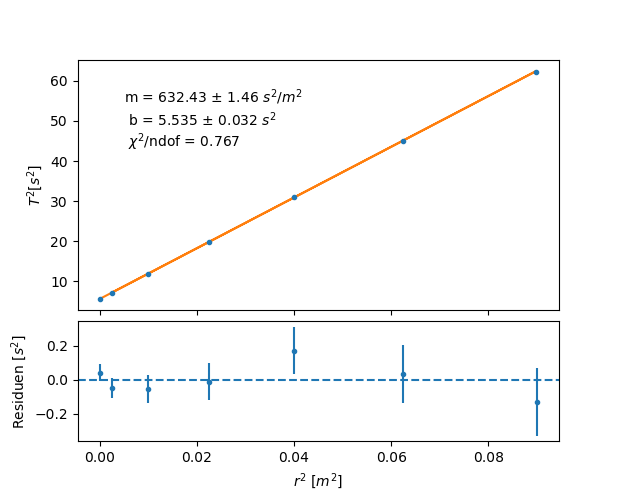
\includegraphics[scale=0.5]{Bilder/Feder2RegD}
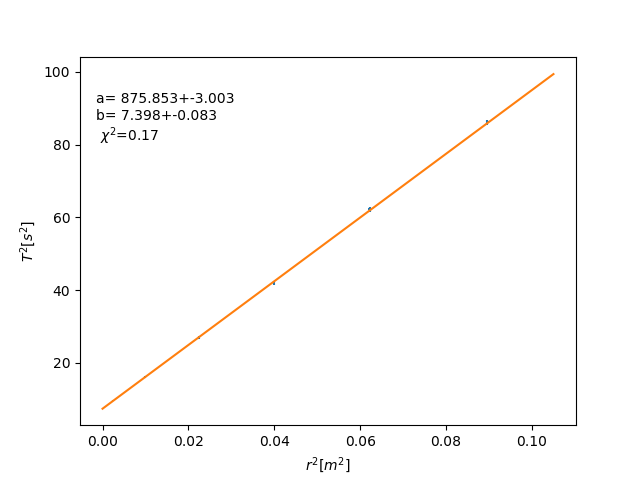
\includegraphics[scale=0.5]{Bilder/Feder3RegD}
\end{center}
\caption{Ergebnisse der Anpassung für Feder 2 (links) und Feder 3 (rechts)}
\label{fig:RegressionenD}
\end{figure}





Mit der Steigung a folgt für das Direktionsmoment
\begin{equation}
D = 4 \pi^2 \frac{m_w}{a} \quad \quad \quad
\sigma_D= D \sqrt{(\frac{\sigma_{m_2}}{m_w})^2+(\frac{\sigma_a}{a})^2}
\end{equation}

wobei $m_w=m_1+m_2$ ist. Die systematischen Fehler der beiden Einzelmassen sind dabei nicht unabhängig und werden linear addiert.\\
Die Ergebnisse der Direktionsmomente finden sich in Tabelle \ref{tab:Direktionsmomente}.

\begin{table}
\caption{Ergebnisse der Direktionsmomentbestimmung}
\begin{center}
\begin{tabular}{|c|c|c|c|}
\hline
Feder & $m_w$[g] & a[$\frac{s^2}{m^2}$] & D[mNm]\\
\hline
2 & 476.00 $\pm$ 0.04 $\pm$ 0.2 & $632.43 \pm 1.46$ & $29.71 \pm 0.07 \pm 0.01$ \\
\hline
3 & 476.90 $\pm$ 0.04 $\pm$ 0.2 & - &  - \\
\hline
\end{tabular}
\end{center}
\label{tab:Direktionsmomente}
\end{table}

Aus dem soeben bestimmten Direktionsmoment und dem y-Achsenabschnitt der Anpassung kann auch das Trägheitsmoment des Stabs ohne angebrachte Massen bestimmt werden und mit dem theoretisch erwarteten Wert verglichen werden.\\

\begin{equation}
J_{Stab}^{exp}=\frac{bD}{4\pi^2} \quad \quad \quad
\sigma_{J_{Stab}^{exp}}=J_{Stab}^{exp} \sqrt{(\frac{\sigma_b}{b})^2+(\frac{\sigma_D}{D})^2}
\end{equation}

Für den Wert aus der Theorie erwartet man

\begin{equation}
J_{Stab}^{theo}=\frac{1}{12} m L^2 \quad \quad \quad
\sigma_{J_{Stab}^{theo}}=\sqrt{(\frac{L^2 \sigma_m}{12})^2+(\frac{2Lm\sigma_L}{12})^2}
\end{equation}

wobei m und L Masse bzw. Länge des Stabs sind.\\
Eine Zusammenstellung der sich so ergebenden Trägheitsmomente findet sich in Tabelle


\begin{table}
\begin{center}
\begin{tabular}{|c|c|c|c|c|}
\hline
Feder & $m_{Stab}$[g] & $L$[cm] & $J_{Stab}^{theo}$[$g m^2$] & $J_{Stab}^{exp}$[$g m^2$]\\
\hline
2 & 131.6 $\pm$ 0.03 $\pm$ 0.1 & 60.9 $\pm$ 0.03 $\pm$ 0.07 & $4.067 \pm 0.004 \pm 0.01 $ & $ 4.165 \pm 0.026 \pm 0.001 $ \\
\hline
3 & 130.5 $\pm$ 0.03 $\pm$ 0.1 & 61.0 $\pm$ 0.03 $\pm$ 0.07 & $4.046 \pm 0.004 \pm  0.01 $ & - \\
\hline
\end{tabular}
\end{center}
\end{table}






\section{Vergleich von Trägheitsmomenten}

\subsection{Auswertung Zylinder}
Bei der Messung der Trägheitsmomente von Hohl- und Vollzylinder wird ein Aufnahmeteller auf die Drillachse gesteckt. Da dieser Teller ein eigenes Trägheitsmoment $J_T$ hat, muss dieses zusätzlich noch bestimmt werden. Dies geschieht über die Aufnahme von Schwingungs-Messungen mit nur dem Teller. Danach werden nacheinander entweder der Voll- oder Hohlzylinder auf den Teller gesteckt und ebenfalls in Schwingung versetzt. Das Trägheitsmoment des Hohlzylinders wird dann folgendermaßen bestimmt:
\begin{equation}
J_{HZ} = J_{gemessen}-J_T
\end{equation}
Analog gilt für den Vollzylinder:
\begin{equation}
J_{VZ} = J_{gemessen}-J_T
\end{equation}
\subsubsection{Rohdaten}
In Abbildung \ref{fig:Teller_Rohdaten} und \ref{fig:Zylinder_Rohdaten} sind zum einen die Rohdaten der Schwingungsmessungen gepltottet. Zum anderen wurde jeweils eine FFT-Transformation zur Veranschaulichung und für eine erste Analyse durchgeführt. Da diese aber zu ungenau ist, wurde mit den FFT-Ergebnissen nicht weitergerechnet.
\begin{figure}
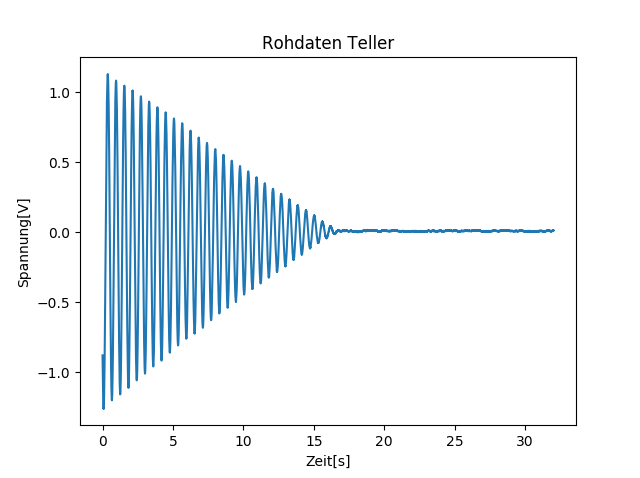
\includegraphics[width=0.49\linewidth]{Bilder/Teller_Rohdaten.PNG}
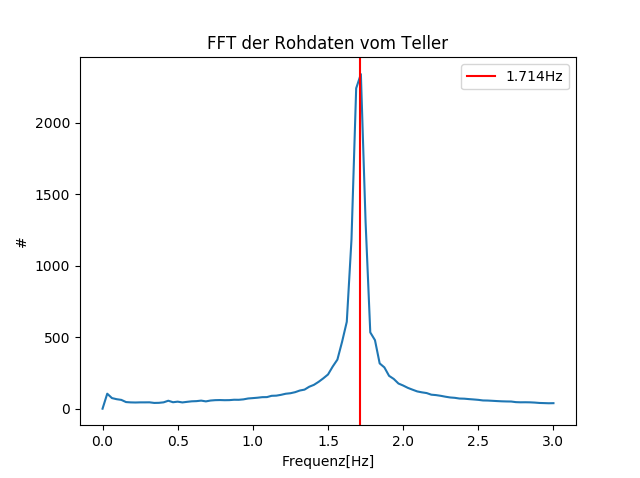
\includegraphics[width=0.49\linewidth]{Bilder/Teller_FFT.PNG}
\caption{Rohdaten der Tellermessung mit FFT zur Veranschaulichung.}
\label{fig:Teller_Rohdaten}
\end{figure}
\begin{figure}
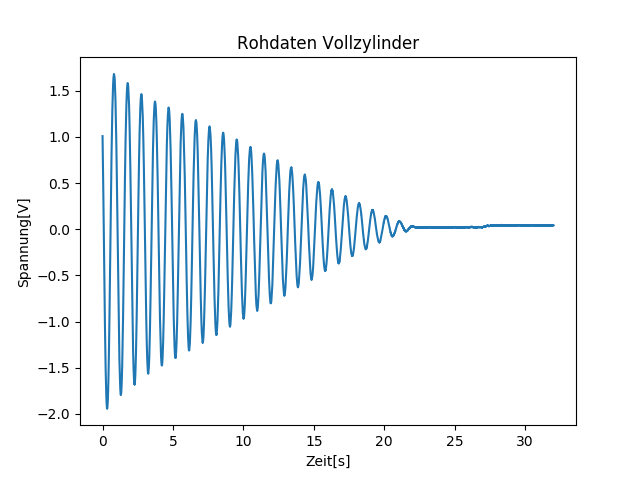
\includegraphics[width=0.49\linewidth]{Bilder/Voll_Rohdaten.PNG}
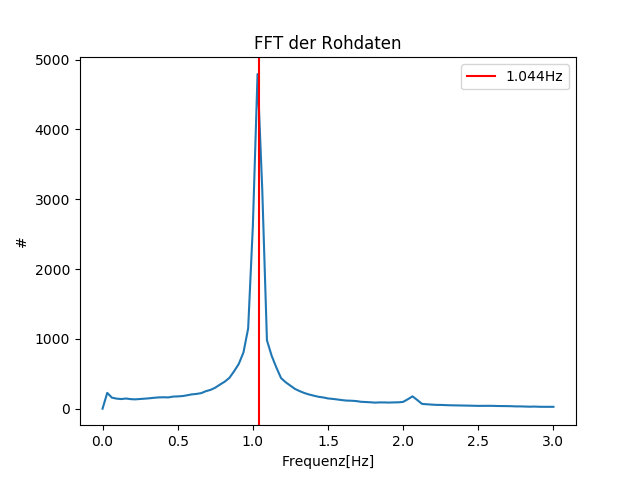
\includegraphics[width=0.49\linewidth]{Bilder/Voll_FFT.PNG}
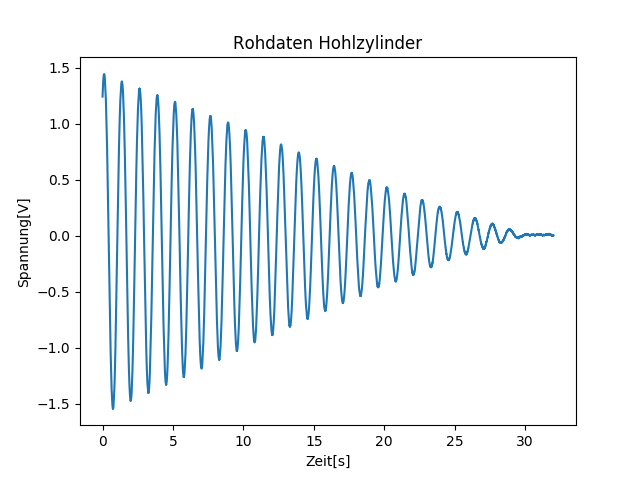
\includegraphics[width=0.49\linewidth]{Bilder/Hohl_Rohdaten.PNG}
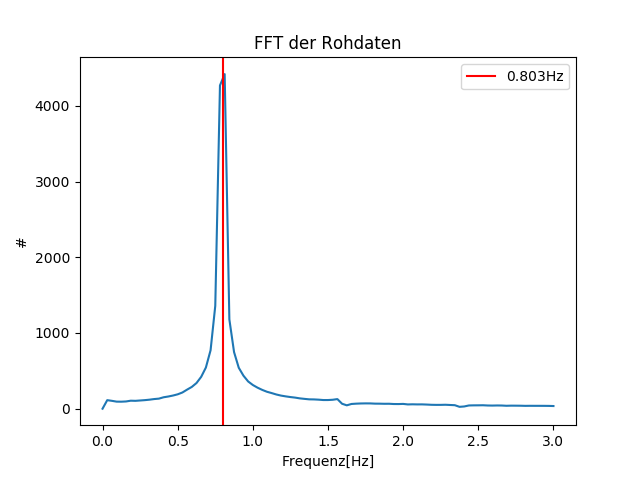
\includegraphics[width=0.49\linewidth]{Bilder/Hohl_FFT.PNG}
\caption{Rohdaten der Zylinder(oben: Vollzylinder, unten: Hohlzylinder) jeweils mit einer FFT zur Veranschaulichung.}
\label{fig:Zylinder_Rohdaten}
\end{figure}

\subsubsection{Messergebnisse}
Um die Periodendauer zu bestimmen, wurden jeweils die Maxima und Minima über eine Periode analysiert. Es wurde also immer die Zeitdifferenz zwischen jedem zweiten Peak bestimmt und anschließend der Mittelwert ausgerechnet. Der Fehler dieser Werte ergibt sich aus dem Fehler auf den Mittelwert.
\begin{table}
\caption{Zwischenergebnisse der Tellermessung.}
\begin{center}
\begin{tabular}{|c|c|c|}
\hline
Messung &  Maxima[s] &  Minima[S]  \\
\hline
0  & $ 0.5857 \pm  0.0005 $ & $ 0.5859 \pm  0.0005 $ \\
\hline
1  & $ 0.5858 \pm  0.0003 $ & $ 0.5858 \pm  0.0004 $ \\
\hline
2  & $ 0.5859 \pm  0.0004 $ & $ 0.5861 \pm  0.0003 $ \\
\hline
3  & $ 0.5862 \pm  0.0003 $ & $ 0.5863 \pm  0.0003 $ \\
\hline
4  & $ 0.5863 \pm  0.0003 $ & $ 0.5865 \pm  0.0004 $ \\
\hline
\end{tabular}
\end{center}
\label{tab:Teller_Ergebnisse}
\end{table}

\begin{table}
\caption{Zwischenergebnisse der Vollzylindermessung.}
\begin{center}
\begin{tabular}{|c|c|c|}
\hline
Messung &  Maxima[s] &  Minima[]  \\
\hline
0  & $ 0.9640 \pm  0.0010 $ & $ 0.9637 \pm  0.0010 $ \\
\hline
1  & $ 0.9650 \pm  0.0009 $ & $ 0.9646 \pm  0.0013 $ \\
\hline
2  & $ 0.9641 \pm  0.0009 $ & $ 0.9643 \pm  0.0010 $ \\
\hline
3  & $ 0.9651 \pm  0.0007 $ & $ 0.9650 \pm  0.0007 $ \\
\hline
4  & $ 0.9641 \pm  0.0009 $ & $ 0.9639 \pm  0.0011 $ \\
\hline
\end{tabular}
\end{center}
\label{tab:Voll_Ergebnisse}
\end{table}

\begin{table}
\caption{Zwischenergebnisse der Hohlzylindermessung.}
\begin{center}
\begin{tabular}{|c|c|c|}
\hline
Messung &  Maxima[s] &  Minima[s]  \\
\hline
1 &  $1.252 \pm 0.001$  &  $1.251 \pm  0.001$ \\
\hline
2 &  $1.252 \pm 0.001$  &  $1.252 \pm  0.001$ \\
\hline
3 &  $1.252 \pm  0.001$  &  $1.252 \pm  0.001$ \\
\hline
3 &  $1.253 \pm  0.001$  &  $1.253 \pm  0.001$ \\
\hline
3 &  $1.253 \pm  0.001$  &  $1.253 \pm  0.001$ \\
\hline
\end{tabular}
\end{center}
\label{tab:Hohl_Ergebnisse}
\end{table}

Die Ergebnisse der fünf Messungen werden nun nochmal durch den Mittelwert zusammengefasst.

\begin{table}
\caption{Endergebnisse der Periodendauer}
\begin{center}
\begin{tabular}{|c|c|}
\hline
Messung &  Ergebnis[s]  \\
\hline
Teller &  $0.5861 \pm 0.0001$ \\
\hline
Vollzylinder &  $0.9638 \pm 0.0004$ \\
\hline
Hohlzylinder &  $1.253 \pm  0.001$ \\
\hline
\end{tabular}
\end{center}
\label{tab:Zylinder_Mittel}
\end{table}
Mit
\begin{equation}
J = \dfrac{D}{4\cdot \pi^{2}}\cdot (T_{VZ/Hz}^{2}-T_T^2)
\end{equation}
kann man nun Das Trägheitsmoment ausrechnen. Die Fehler berechnen sich aus der Gausschen Fehlerfortpflanzung:
\begin{equation}
\sigma_J = \sqrt{(\dfrac{1}{4\cdot \pi^{2}}\cdot (T_{VZ/Hz}^{2}-T_T^2)\cdot \sigma_D )^2+ (\dfrac{2}{4\cdot \pi^{2}}\cdot T_{VZ/Hz}\cdot \sigma_{T(VZ/Hz)})^2+ (\dfrac{2}{4\cdot \pi^{2}}\cdot T_{T}\cdot \sigma_{TT} )^2}
\end{equation}

\begin{table}
\caption{Bestimmte Trägheitsmomente}
\begin{center}
\begin{tabular}{|c|c|c|c|}
\hline
Messung &  Ergebnis[$gm^2$] & Theorie & Standardabweichungen \\
\hline
Teller &  $0.1741 \pm 0.0001$ & &\\
\hline
Vollzylinder &  $0.3226 \pm 0.0004\pm 0.0057$ & $0.3226\pm 0.0001\pm 0.0007$ & 0.007\\
\hline
Hohlzylinder &  $0.6760 \pm 0.0016\pm 0.0119$ & $0.6759\pm 0.0001\pm 0.0031$ & 0.006\\
\hline
\end{tabular}
\end{center}
\label{tab:Zylinder_Mittel}
\end{table}

\subsection{Auswertung Kugel und Scheibe}
Der Aufbau mit dem die Kugel und die Scheibe vermessen wurden, enthielt die Feder Nummer 2. \\
Für die Messung des Trägheitsmomentes der Kugel, wird die Kugel direkt auf die Drillachse gesteckt. Der Teller wird hierbei also nicht benötigt. Das Trägheitsmoment der Drillachse liegt in der Größenordnung $10^{-5} \dfrac{kg}{m \cdot s^2}$ und wird daher ebenfalls vernachlässigt. Ob dies eine sinnvolle Näherung ist, muss im Anschluss anhand des Ergebnisses überprüft werden. \\
Der Literaturwert berechnet sich zu:
\begin{equation}
J_K^{theo} = \dfrac{2}{5} \cdot m_K \cdot R_K^2
\label{eq:JKtheo}
\end{equation}
\begin{equation}
J_S^{theo} = \dfrac{1}{2} \cdot m_S \cdot R_S^2
\label{eq:JStheo}
\end{equation}
Dazu müssen die Kugel gewogen und der Durchmesser der Kugel gemessen werden. Die Fehler auf diese Messungen pflanzen sich folgendermaßen fort:
\begin{equation}
\sigma_{J_K^{theo}} = \dfrac{2}{5} \cdot \sqrt{\left( \sigma_{m_K} \cdot R_K^2 \right)^2 + \left( \sigma_{R_K} \cdot 2 \cdot m_K \cdot R_K \right)^2}
\label{eq:sigJKtheo}
\end{equation}
\begin{equation}
\sigma_{J_S^{theo}} = \dfrac{1}{2} \cdot \sqrt{\left( \sigma_{m_S} \cdot R_S^2 \right)^2 + \left( \sigma_{R_S} \cdot 2 \cdot m_S \cdot R_S \right)^2}
\label{eq:sigJKtheo}
\end{equation}
Das Trägheitsmoment wird über die Schwingung des Körpers auf einer Spiralfeder bestimmt. Misst man die Periodendauer für eine Spiralfeder mit bekanntem Direktionsmoment, kann man das Trägheitsmoment mit Gleichung \ref{eq:Trägheitsmoment} berechnen. Der Fehler auf das Trägheitsmoment ergibt sich dann nach gauß'scher Fehlerfortpflanzung zu:
\begin{equation}
\sigma_J = \dfrac{1}{4 \cdot \pi^2} \cdot \sqrt{ \left( \sigma_D \cdot T^2 \right)^2 + \left( \sigma_T \cdot 2 \cdot D \cdot T \right)^2}
\label{eq:sigTrägheitsmoment}
\end{equation}

\subsubsection{Rohdaten}
\begin{figure}
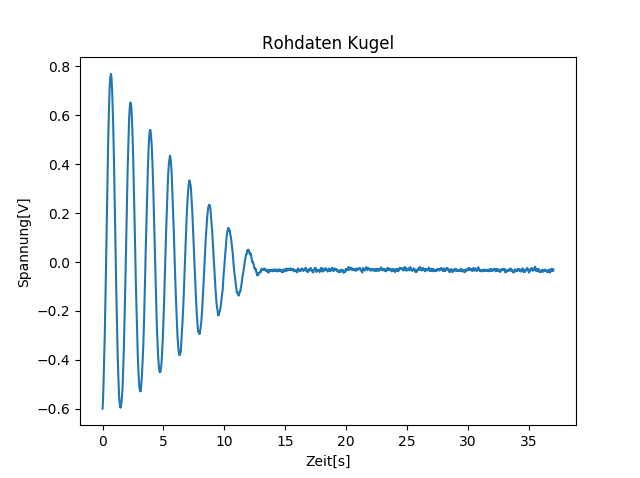
\includegraphics[width=0.49\linewidth]{Bilder/Kugel_Rohdaten.PNG}
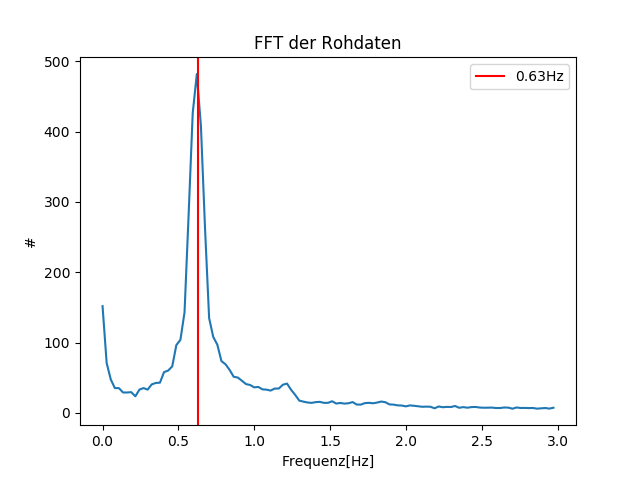
\includegraphics[width=0.49\linewidth]{Bilder/Kugel_FFT.PNG}
\caption{Rohdaten der Kugelmessung mit FFT zur Veranschaulichung.}
\label{fig:Kugel_Rohdaten}
\end{figure}
\begin{figure}
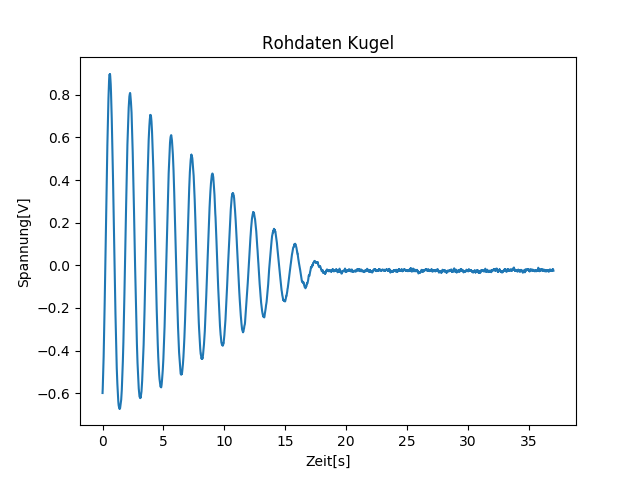
\includegraphics[width=0.49\linewidth]{Bilder/Scheibe_Rohdaten.PNG}
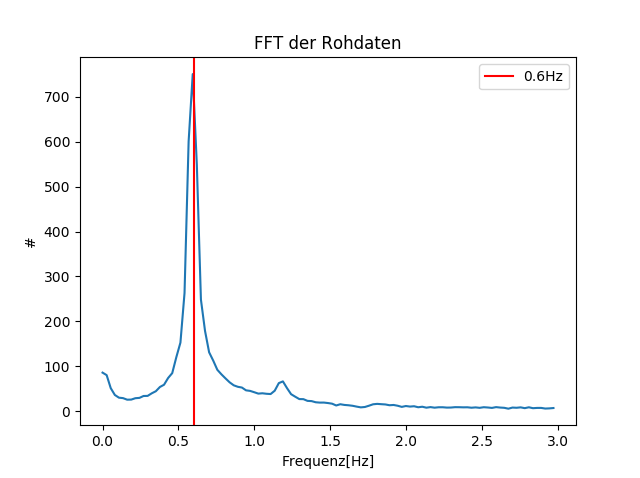
\includegraphics[width=0.49\linewidth]{Bilder/Scheibe_FFT.PNG}
\caption{Rohdaten der Scheibenmessung mit FFT zur Veranschaulichung.}
\label{fig:Scheibe_Rohdaten}
\end{figure}
Abbildung \ref{fig:Kugel_Rohdaten} zeigt die Rohdaten der Messung des Trägheitmomentes der Kugel sowie eine FFT der Daten zur Veranschaulichung. Abbildung \ref{fig:Scheibe_Rohdaten} zeigt das Analogon dazu für die Messung der Scheibe. Die FFT wurde in der Auswertung nicht verwendet, da die Auflösung zu gering ist und deswegen einen zu großen Fehler auf die Messung der Periodendauer liefert.

\subsubsection{Auswertung}
Wegen der nicht hinreichend genauen FFT wurde die Periodendauer durch Abzählen der Extrema bestimmt. Dabei werden die Extrema abgezählt und anschließend die doppelte Zeitdifferenz zwischen dem ersten und letzten Extremum durch die Zahl der Extrema geteilt. Tabelle \ref{tab:Kugel_Periodendauern} zeigt die Ergebnisse der Mehrfachmessungen.

\begin{table}
\caption{Mehrfachmessung der Periodendauer für Kugel}
\label{tab:Kugel_Periodendauern}
\begin{center}
\begin{tabular}{|c|c|c|c|}
\hline 
Messung & Anzahl Extrema & Zeitdifferenz [s] & Errechnete Periodendauer [s] \\ 
\hline 
1 & 13 & 9,685 & 1,6142 \\ 
\hline 
2 & 13 & 9,68 & 1,6133 \\ 
\hline 
3 & 13 & 9,69 & 1,6150 \\ 
\hline 
4 & 13 & 9,69 & 1,6150 \\ 
\hline 
5 & 13 & 9,69 & 1,6150 \\ 
\hline 
6 & 13 & 9,69 & 1,6150 \\ 
\hline 
7 & 13 & 9,685 & 1,6142 \\ 
\hline 
8 & 13 & 9,685 & 1,6142 \\ 
\hline 
9 & 13 & 9,685 & 1,6142 \\ 
\hline 
10 & 13 & 9,68 & 1,6133 \\ 
\hline 
\end{tabular} 
\end{center}
\end{table}

\begin{table}
\caption{Mehrfachmessung der Periodendauer für Scheibe}
\label{tab:Scheibe_Periodendauern}
\begin{center}
\begin{tabular}{|c|c|c|c|}
\hline 
Messung & Anzahl Extrema & Zeitdifferenz [s] & Errechnete Periodendauer [s] \\ 
\hline 
1 & 14 & 10,99 & 1,6908 \\ 
\hline 
2 & 14 & 10,945 & 1,6838 \\ 
\hline 
3 & 14 & 10,98 & 1,6892 \\ 
\hline 
4 & 14 & 10,985 & 1,6900 \\ 
\hline 
5 & 14 & 10,99 & 1,6908 \\ 
\hline 
6 & 14 & 10,985 & 1,6900 \\ 
\hline 
7 & 14 & 10,98 & 1,6892 \\ 
\hline 
8 & 14 & 10,98 & 1,6892 \\ 
\hline 
9 & 14 & 10,975 & 1,6885 \\ 
\hline 
10 & 14 & 10,98 & 1,6892 \\ 
\hline 
\end{tabular} 
\end{center}
\end{table}

Aus der Mehrfachmessung lässt sich nun ein empirischer Mittelwert und eine empirische Standardabweichung bestimmen:
\[\overline{T_K} = 1,6143 \,s \quad \sigma_{T_K} = 0,0020 \, s \]
\[\overline{T_S} = 1,6891 \, s \quad \sigma_{T_S} = 0,0043 \, s \]
Damit lässt nun das Endergebnis für das Trägheitsmoment und dessen Fehler berechnen:
\[J_K^{exp} = (1,9612 \pm 0,0049 \pm 0,0045) \, \si{g.m ^2} \]
\[J_S^{exp} = (2,1473 \pm 0,0109 \pm 0,0154) \, \si{g.m ^2} \]
Hieran lässt sich nun gut ersehen, dass die Vernachlässigung des Trägheitsmomentes der Drillachse (Größenordnung $0,01\si{g.m ^2}$) gerechtfertigt war, da das Trägheitmoment der Kugel zwei Größenordnungen größer ist und das Trägheitsmoment der Drillachse damit keinen relevanten Beitrag liefert.

\subsubsection{Fazit}
Das theoretische Trägheitsmoment der Kugel und dessen Fehler errechnet sich mit Gleichungen \ref{eq:JKtheo} und \ref{eq:sigJKtheo} zu:
\[J_K^{theo} = (1,8859 \pm 0,0289 \pm 0,0038) \, \si{g.m ^2} \]
\[J_S^{theo} = (2,1049 \pm 0,0054 \pm 0,0043) \, \si{g.m ^2} \]
Die Abweichung $\Delta$ des experimentellen Wertes vom theoretischen Wert beträgt damit 
\[\dfrac{\Delta}{\sigma _K^{exp}} = \dfrac{J_K^{exp} - J_K^{theo} - \sqrt{\left( \sigma _K^{sys,theo}\right) ^2 + \left( \sigma _K^{stat,theo}\right) ^2}}{\sigma _K^{exp}} = 3,3 \]
\[\dfrac{\Delta}{\sigma _S^{exp}} = \dfrac{J_S^{exp} - J_S^{theo} - \sqrt{\left( \sigma _S^{sys,theo}\right) ^2 + \left( \sigma _S^{stat,theo}\right) ^2}}{\sigma _S^{exp}} = 2,3 \]
Damit liegt der gemessene Wert so gerade noch in einem akzeptablen Rahmen. \\
Außerdem liegen die Trägheitsmomente mit nur etwa 8,7\% Abweichung wie erwartet sehr nah beieinander.




\section{Bestätigung des Steinerschen Satzes}
\subsection{Beschreibung}
Zur Bestätigung des Steinerschen Satzes werden die Quadrate der Periodendauern gegen die Quadrate der Verschiebung des Schwerpunktes zur 
Drehachse aufgetragen.\\
Dabei gilt:

\begin{equation}
\sigma_{T^2}=2 T \sigma_T \quad \quad \quad
\sigma_{r^2}=2r \sigma_r
\end{equation}

Die Periodendauer T ist dabei der Mittelwert von Mehrfachmessungen für jede Einstellungen, der Fehler ist der Fehler auf den Mittelwert der sich aus dieser Stichprobe ergibt.\\
Da der Kerbenabstand d bekannt ist erhält man für den Abstand der Dreh- zur Schwerpunktsachse r mit $r = n \cdot d$:
\begin{equation}
\sigma_{r,stat.}=\sqrt{n} \sigma_{d,stat.} \quad \text{n ist dabei die Position der Kerbe von der Mitte aus gezählt}
\end{equation}

Der systematische Fehler der Längenmessung ist bei Addition der Kerbenabstände nicht unabhängig und wird deswegen linear und nicht quadratisch addiert. Es folgt:

\begin{equation}
\sigma_{r,syst.}=n \sigma_{d,syst.}
\end{equation}

Für die Steigungen a gilt hier der Zusammenhang:
\begin{equation}
a=\frac{4\pi^2 m}{D}
\end{equation}

Damit kann aus der Steigung mithilfe des zuvor bestimmten Direktionsmoments die Masse des Stabs abgeschätzt und mit dem experimentell ermittelten Wert verglichen werden.\\

\subsection{Rohdaten}
An den so transformierten Daten wurde für beide Federn eine lineare Regression durchgeführt. Die Ergebnisse befinden sich in Abbildung \ref{fig:SteinerReg2} bzw. Abbildung \ref{fig:SteinerReg3}.

\begin{figure}
\begin{center}
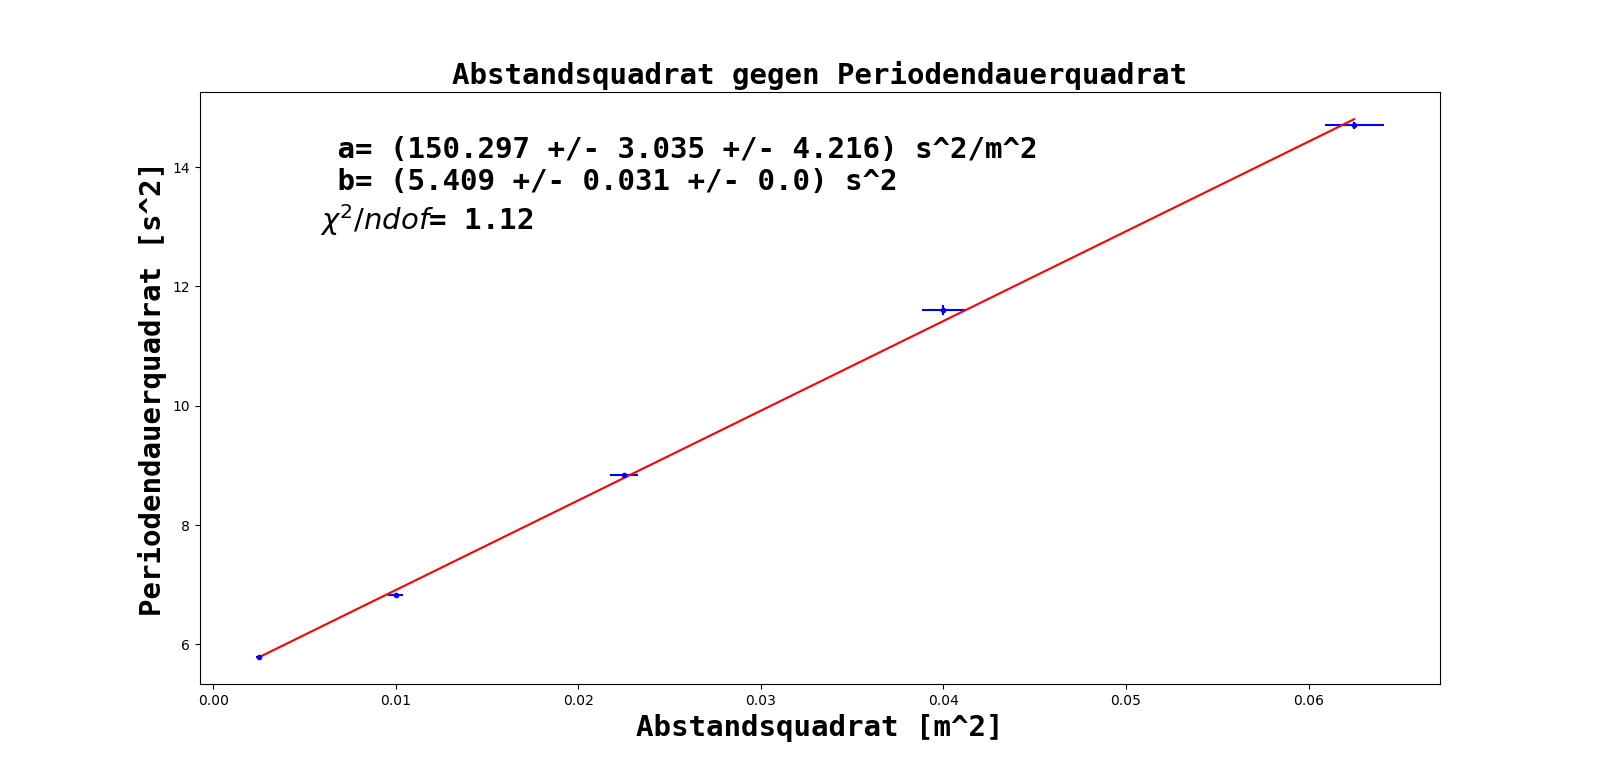
\includegraphics[scale=0.3]{Bilder/Steiner_Feder2_linReg}
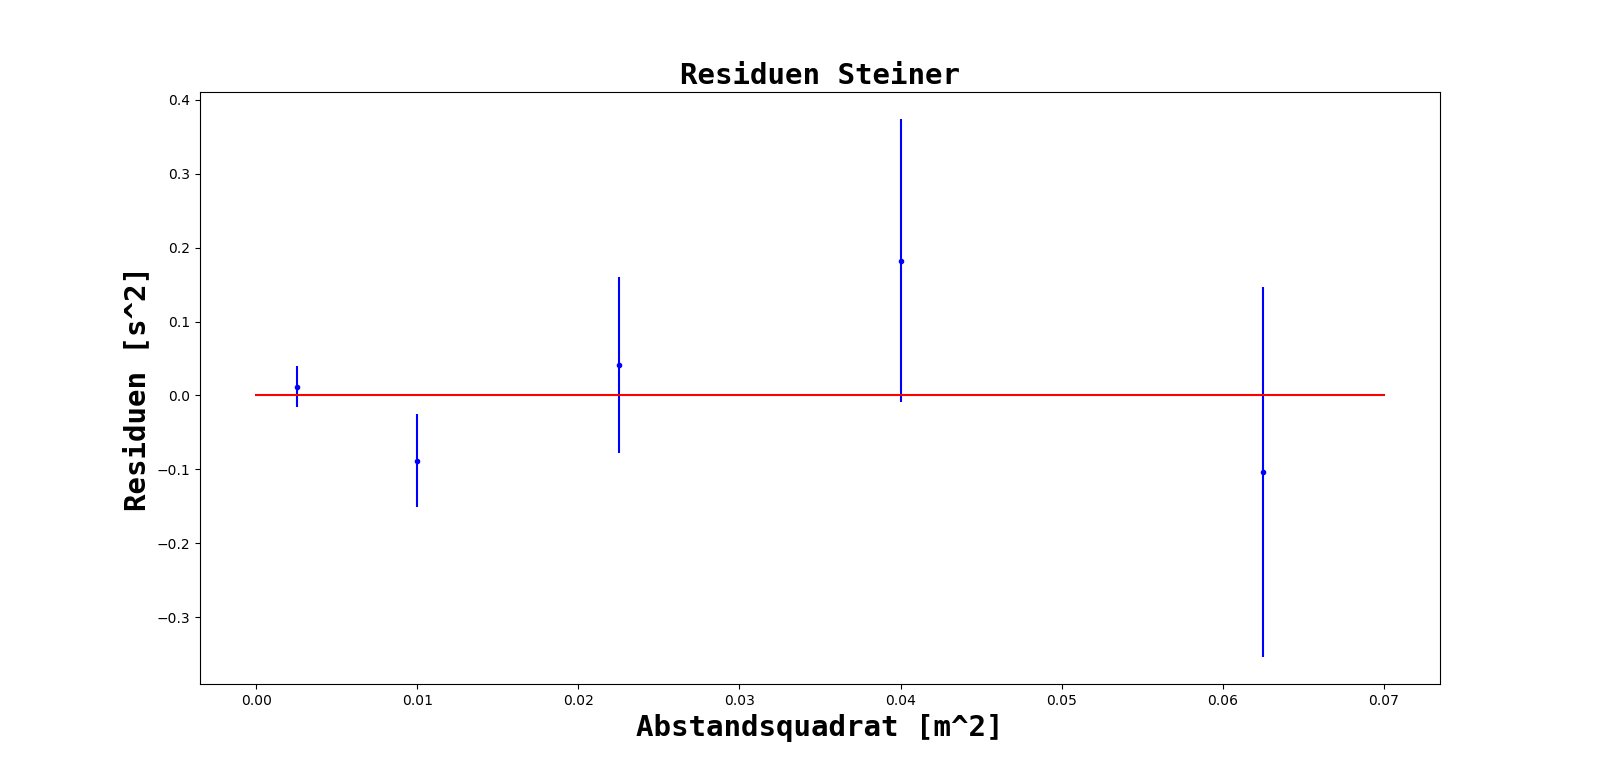
\includegraphics[scale=0.3]{Bilder/Steiner_Feder2_Residuen}
\end{center}
\caption{Regressionsergebnisse für Feder 2}
\label{fig:SteinerReg2}
\end{figure}

\begin{figure}
\begin{center}
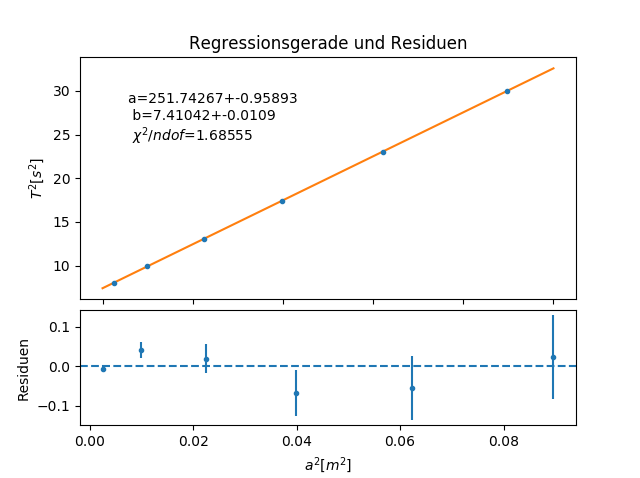
\includegraphics[scale=0.8]{Bilder/SteinerFeder3Komplett}
\end{center}
\caption{Regressionsergebnisse für Feder 3}
\label{fig:SteinerReg3}
\end{figure}

\subsection{Auswertung}


hier dann blabla, umrechnen, vergleichen und fehler erklären mit das das nicht perfekt gelagert war blabla





\end{document}